\chapter{Introduction}
\Jnote{Please read the text again and correct language mistakes.
  Also pay attention to punctuation.}
\section*{1.1. Introduction}
In every organization there is a way to communicate ,one of the most popular way to transmit the information  is  to produce a written report which explains how different activities of the organization are going. For the large organizations there a huge number of reports, imagine the way it is challenging go through  each and every report manually.
\Jnote{``imagine the way...'' This is not good language for a research essay.}
This research has an aim of providing an easy way of visualizing and extracting the important information locked in reports from NGO and large organisations.
In 1919, The International Federation of Red Cross and Red Crescent societies (IFRC) has been founded, it has some millions of reports related to humanitarian support,How to  know automatically the number of people who suffered from a disease, How to know the  fraction of fund spent on shelter ?  In this research, There are some solutions to those questions by using combination of statistics and Natural Language Processing (NLP)techniques.
Big data and Machine learning is for analysing the huge data by using statistical and computing algorithms. Document modelling by extracting entities is one of the way to deal with natural big data linguistic problems where entity is defined as a single unit of data, it can be classified based on its relationship, Entity can be location , people, organization and so one.

\Jnote{Paragraph above has many topics (organizing information, Red Cross,
  NLP, document modelling) mixed together. Please separate them into
  paragraphs.}

Let MDRAF003 be IFRC report "Afghanistan MDRAF003 26May2016.pdf", it is composed by 12 pages of texts.
\Jnote{s/Let MDRAF003.../For example, consider an IFRC report...}
To extract entities  from MDRAF003 is challenging, what are the key points to be performed?
\begin{itemize}
\item The sentences which compose a report  must be parsed.
\item  Entities also must be identified in the report
\item Relationship between entities must be modelled.
\end{itemize}
In this research, there is a clear discussion about powerful techniques to answer the previous questions.  Natural  Language Processing techniques used to sentence level and content based analysis,Natural Language ToolKit  (NLTK) for spliting the sentences into tokens and remove the common words and how to work with corpus.The used reports for the implementation of different language algorithms are from IFRC .

\section*{1.2. Motivation}
Big data and Machine learning have recently become one of the major and strong solution finder to most difficult problems in heath, statistical prediction, company development and linguistics.Big data is a future for everything.
\Jnote{``Big data is a future for everything.'' This sentence does not really
  say anything. I would avoid writing sentences like this.}
within huge reports,journals or articles ,this work will return significant  classified entities which will help the user to not struggle opening the report and get like amount spent in a given activity, the sum of people who participated in an event etc.




% =======================
%
%This is a textual citation \citet{shannon44}. And this is a parenthetical citation \citep{shannon44}. You probably want to use the latter more often.
%\begin{figure}[!h]
%% Use "\centering" in floats (figure, table), but if you need to center
%% some text (why?) use "\begin{center}...\end{center}".
%\centering 
%% Figure environments same as 0.8 * \textwidth please
%% That does not necessarily mean the actual picture size,
%% it is a guideline for the environment which could contain
%% 2 or more pictures! Be consistent and follow the guidelines
%% provided in your sources.
%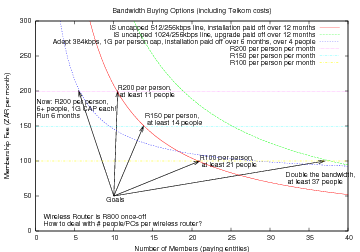
\includegraphics[width=0.8\textwidth]{images/bandwidth-colour.png}
%\caption{Planning community bandwidth sharing costs. 
%  Note caption capitalization.}
% 
%\label{bandwidth} 
%% if you move the label it breaks the reference numbering; 
%% always have it *after* the caption.
%\end{figure}
%Remember how to include code with {\tt verbatim} 
%and to fix the tabs in {\sf python} in a verbatim environment? 
%It may be best to have an `include' command for code, 
%not to have to re-edit it all the time.
%\verbatimtabinput{code/mycode.py}
%=======================

